\documentclass[14pt]{extbook}
\usepackage{multicol, enumerate, enumitem, hyperref, color, soul, setspace, parskip, fancyhdr} %General Packages
\usepackage{amssymb, amsthm, amsmath, latexsym, units, mathtools} %Math Packages
\everymath{\displaystyle} %All math in Display Style
% Packages with additional options
\usepackage[headsep=0.5cm,headheight=12pt, left=1 in,right= 1 in,top= 1 in,bottom= 1 in]{geometry}
\usepackage[usenames,dvipsnames]{xcolor}
\usepackage{dashrule}  % Package to use the command below to create lines between items
\newcommand{\litem}[1]{\item#1\hspace*{-1cm}\rule{\textwidth}{0.4pt}}
\pagestyle{fancy}
\lhead{Progress Quiz 6}
\chead{}
\rhead{Version B}
\lfoot{4563-7456}
\cfoot{}
\rfoot{Summer C 2021}
\begin{document}

\begin{enumerate}
\litem{
Choose the graph of the equation below.\[ f(x) = \frac{1}{(x - 1)^2} + 1 \]\begin{enumerate}[label=\Alph*.]
\begin{multicols}{2}\item 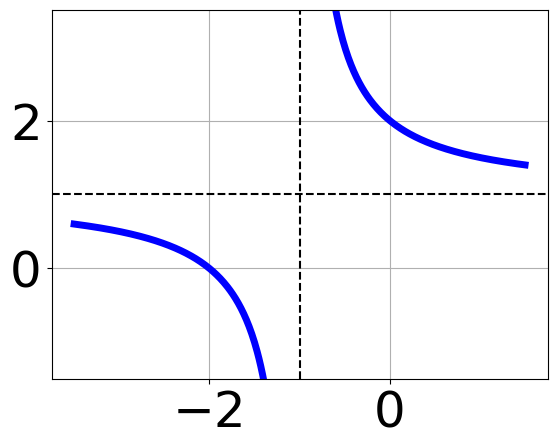
\includegraphics[width = 0.3\textwidth]{../Figures/rationalEquationToGraphAB.png}\item 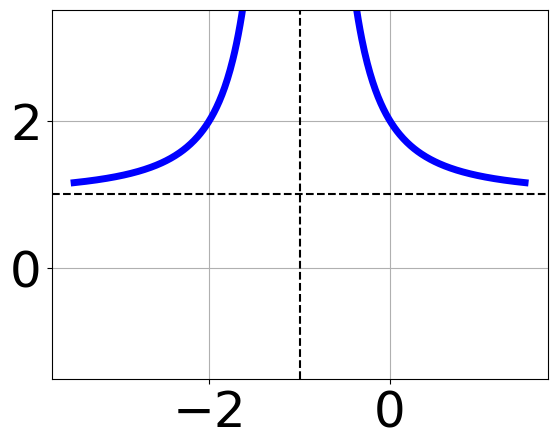
\includegraphics[width = 0.3\textwidth]{../Figures/rationalEquationToGraphBB.png}\item 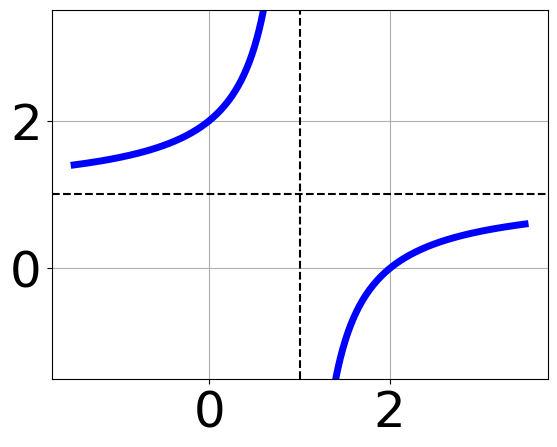
\includegraphics[width = 0.3\textwidth]{../Figures/rationalEquationToGraphCB.png}\item 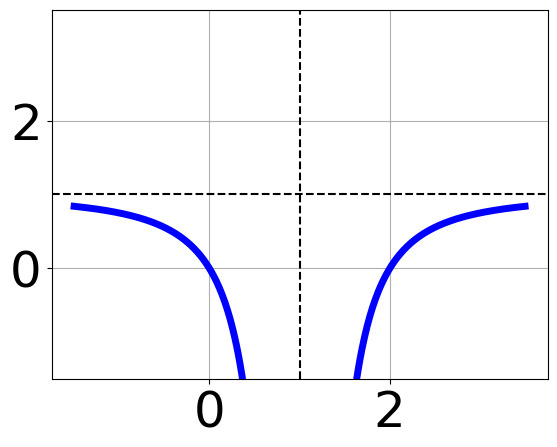
\includegraphics[width = 0.3\textwidth]{../Figures/rationalEquationToGraphDB.png}\end{multicols}\item None of the above.
\end{enumerate} }
\litem{
Choose the equation of the function graphed below.
\begin{center}
    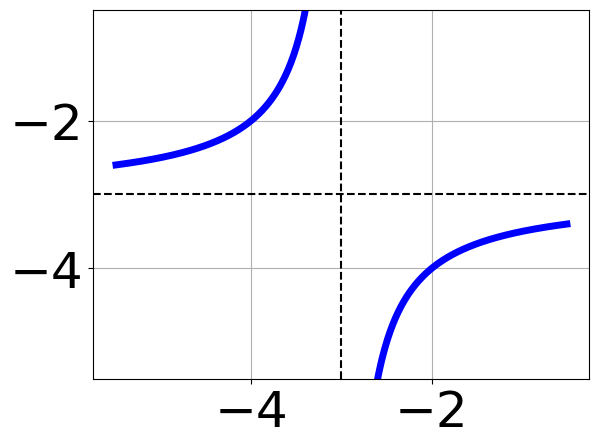
\includegraphics[width=0.5\textwidth]{../Figures/rationalGraphToEquationB.png}
\end{center}
\begin{enumerate}[label=\Alph*.]
\item \( f(x) = \frac{1}{(x - 3)^2} - 4 \)
\item \( f(x) = \frac{1}{x - 3} - 4 \)
\item \( f(x) = \frac{-1}{x + 3} - 4 \)
\item \( f(x) = \frac{-1}{(x + 3)^2} - 4 \)
\item \( \text{None of the above} \)

\end{enumerate} }
\litem{
Solve the rational equation below. Then, choose the interval(s) that the solution(s) belongs to.\[ \frac{5x}{5x -7} + \frac{-3x^{2}}{-20x^{2} +43 x -21} = \frac{-4}{-4x + 3} \]\begin{enumerate}[label=\Alph*.]
\item \( x_1 \in [1.73, 2.02] \text{ and } x_2 \in [0.03,0.4] \)
\item \( \text{All solutions lead to invalid or complex values in the equation.} \)
\item \( x_1 \in [1.08, 1.47] \text{ and } x_2 \in [0.57,0.79] \)
\item \( x \in [1.08,1.47] \)
\item \( x \in [-0.56,0.93] \)

\end{enumerate} }
\litem{
Solve the rational equation below. Then, choose the interval(s) that the solution(s) belongs to.\[ \frac{72}{18x + 18} + 1 = \frac{72}{18x + 18} \]\begin{enumerate}[label=\Alph*.]
\item \( \text{All solutions lead to invalid or complex values in the equation.} \)
\item \( x_1 \in [-1, 0] \text{ and } x_2 \in [-1,0] \)
\item \( x \in [0,3] \)
\item \( x_1 \in [-1, 0] \text{ and } x_2 \in [1,2] \)
\item \( x \in [-1.0,0.0] \)

\end{enumerate} }
\litem{
Choose the equation of the function graphed below.
\begin{center}
    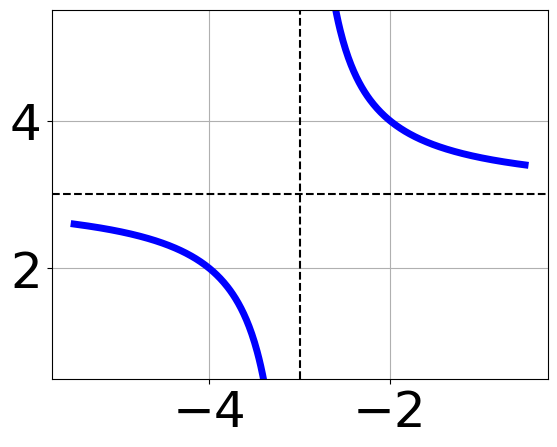
\includegraphics[width=0.5\textwidth]{../Figures/rationalGraphToEquationCopyB.png}
\end{center}
\begin{enumerate}[label=\Alph*.]
\item \( f(x) = \frac{1}{(x + 3)^2} + 3 \)
\item \( f(x) = \frac{-1}{(x - 3)^2} + 3 \)
\item \( f(x) = \frac{1}{x + 3} + 3 \)
\item \( f(x) = \frac{-1}{x - 3} + 3 \)
\item \( \text{None of the above} \)

\end{enumerate} }
\litem{
Solve the rational equation below. Then, choose the interval(s) that the solution(s) belongs to.\[ \frac{-8}{-6x + 2} + -9 = \frac{-9}{48x -16} \]\begin{enumerate}[label=\Alph*.]
\item \( x \in [0.5,2.5] \)
\item \( x_1 \in [-0.29, 0.02] \text{ and } x_2 \in [-1.5,3.5] \)
\item \( \text{All solutions lead to invalid or complex values in the equation.} \)
\item \( x \in [-0.29,0.02] \)
\item \( x_1 \in [0.09, 0.41] \text{ and } x_2 \in [-1.5,3.5] \)

\end{enumerate} }
\litem{
Choose the graph of the equation below.\[ f(x) = \frac{1}{x + 2} - 2 \]\begin{enumerate}[label=\Alph*.]
\begin{multicols}{2}\item 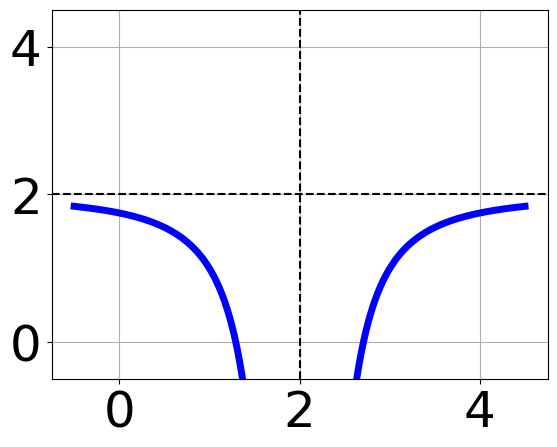
\includegraphics[width = 0.3\textwidth]{../Figures/rationalEquationToGraphCopyAB.png}\item 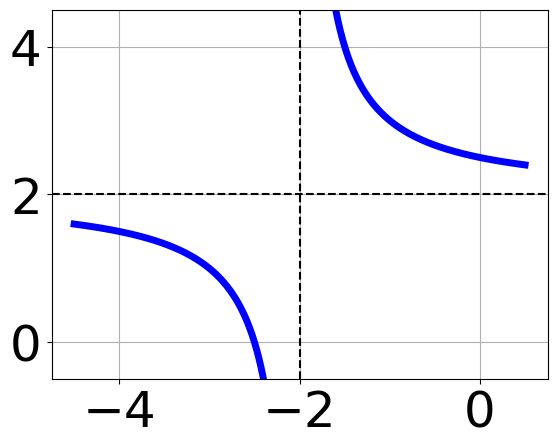
\includegraphics[width = 0.3\textwidth]{../Figures/rationalEquationToGraphCopyBB.png}\item 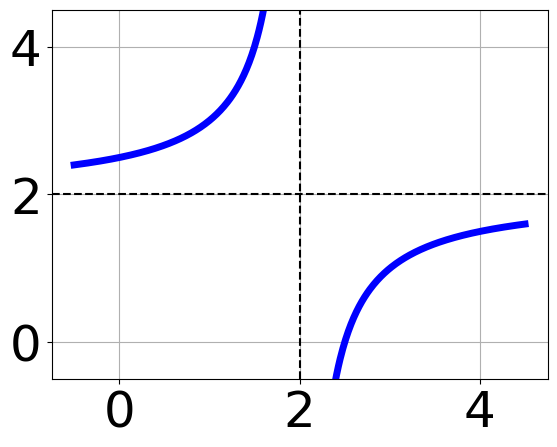
\includegraphics[width = 0.3\textwidth]{../Figures/rationalEquationToGraphCopyCB.png}\item 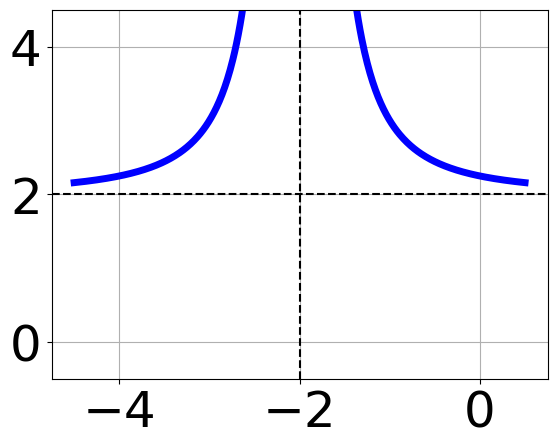
\includegraphics[width = 0.3\textwidth]{../Figures/rationalEquationToGraphCopyDB.png}\end{multicols}\item None of the above.
\end{enumerate} }
\litem{
Determine the domain of the function below.\[ f(x) = \frac{4}{20x^{2} -54 x + 36} \]\begin{enumerate}[label=\Alph*.]
\item \( \text{All Real numbers.} \)
\item \( \text{All Real numbers except } x = a \text{ and } x = b, \text{ where } a \in [23.82, 24.02] \text{ and } b \in [29.77, 30.1] \)
\item \( \text{All Real numbers except } x = a, \text{ where } a \in [23.82, 24.02] \)
\item \( \text{All Real numbers except } x = a \text{ and } x = b, \text{ where } a \in [0.78, 1.31] \text{ and } b \in [1.33, 1.73] \)
\item \( \text{All Real numbers except } x = a, \text{ where } a \in [0.78, 1.31] \)

\end{enumerate} }
\litem{
Determine the domain of the function below.\[ f(x) = \frac{3}{12x^{2} -42 x + 36} \]\begin{enumerate}[label=\Alph*.]
\item \( \text{All Real numbers except } x = a, \text{ where } a \in [17.7, 20.1] \)
\item \( \text{All Real numbers.} \)
\item \( \text{All Real numbers except } x = a \text{ and } x = b, \text{ where } a \in [0, 1.6] \text{ and } b \in [1.8, 2.3] \)
\item \( \text{All Real numbers except } x = a, \text{ where } a \in [0, 1.6] \)
\item \( \text{All Real numbers except } x = a \text{ and } x = b, \text{ where } a \in [17.7, 20.1] \text{ and } b \in [22.7, 24.9] \)

\end{enumerate} }
\litem{
Solve the rational equation below. Then, choose the interval(s) that the solution(s) belongs to.\[ \frac{-4x}{3x + 3} + \frac{-2x^{2}}{-21x^{2} -12 x + 9} = \frac{7}{-7x + 3} \]\begin{enumerate}[label=\Alph*.]
\item \( x_1 \in [-0.53, -0.32] \text{ and } x_2 \in [-1.3,-0.4] \)
\item \( \text{All solutions lead to invalid or complex values in the equation.} \)
\item \( x_1 \in [-0.53, -0.32] \text{ and } x_2 \in [0.1,1.9] \)
\item \( x \in [0.36,0.88] \)
\item \( x \in [1.51,2.18] \)

\end{enumerate} }
\end{enumerate}

\end{document}